\section{研究背景与设计目标}

\subsection{从“看起来标准”到“真的练到了”}

居家健身系统近几年越来越常见，但大多数产品仍然把核心能力放在摄像头
姿态识别上。这个方向有其合理性：摄像头便宜、安装简单，人体骨架检测模型
也已经相对成熟。它能判断膝盖有没有内扣、手臂有没有抬到位、动作幅度
是否够大，因此适合承担第一层动作反馈。

问题在于，健身动作不只是一条外部轨迹。两个人做出几乎相同的深蹲姿态，
一个可能主要由股四头肌和臀肌发力，另一个可能更多依赖关节代偿和代偿肌
完成动作。
在摄像头眼里，这两种动作可能差别不大；但从训练效果和损伤风险看，它们
并不是同一类动作。也就是说，纯视觉系统能看到“形”，却看不到“力”。

\begin{figure}[htbp]
    \centering
    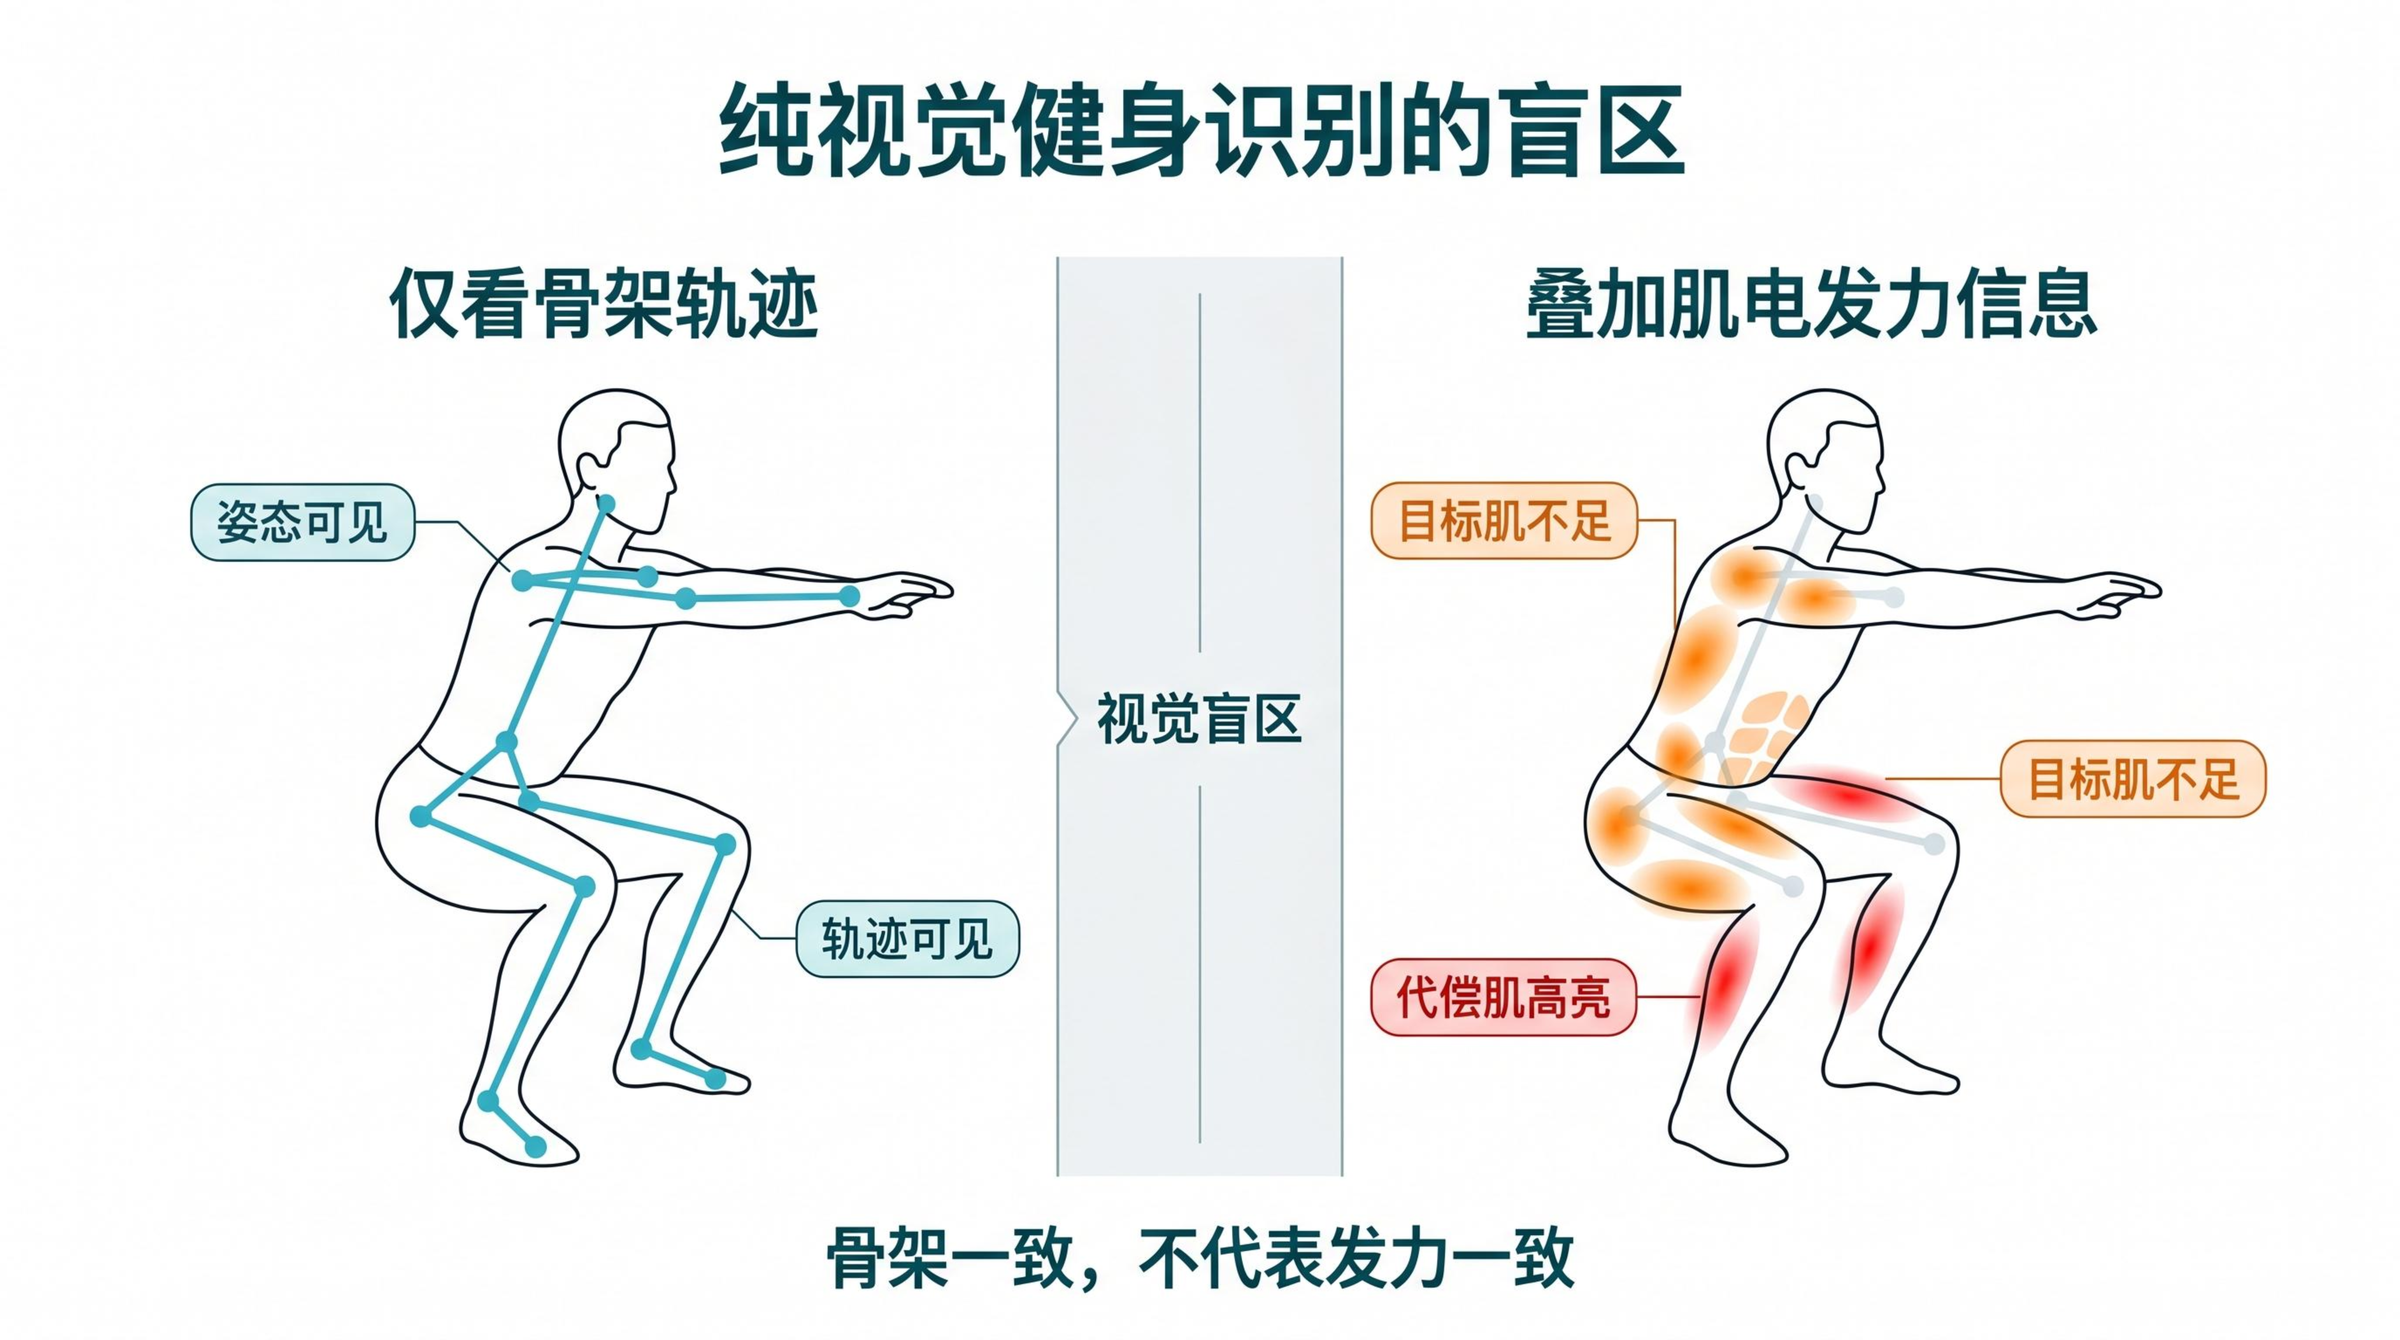
\includegraphics[width=0.88\textwidth]{figures/report/fig01.png}
    \caption{视觉姿态与肌电发力信息的互补关系示意。}
    \label{fig:vision-blind-spot}
\end{figure}

表面肌电（surface EMG, sEMG）提供了另一条观察路径。电极贴在皮肤表面
后，可以采集肌肉收缩时产生的微弱电信号。它不能替代视觉，因为肌电本身
不知道身体姿态；但它可以补上视觉看不到的肌肉激活信息。本项目的
核心想法就是把这两类信息放在一起：视觉负责看动作阶段和外部轨迹，肌电
负责看目标肌肉和代偿肌肉的实际参与程度。

\subsection{项目希望解决的三个问题}

围绕这个出发点，本项目最终要解决的不是单点算法问题，而是一条完整
的嵌入式系统链路。

\begin{enumerate}
    \item \term{感知问题}：如何同时拿到视觉姿态和肌电信号，并让它们在
    同一组动作里对齐。视觉帧率、肌电采样频率和动作周期都不一样，直接
    把原始数据拼在一起并不现实。

    \item \term{判断问题}：如何判断一次动作到底是标准、不标准，还是
    发生了代偿。这个判断不能只靠硬编码阈值，否则每换一个动作、一个人
    或一套贴片位置，都需要重新调参数。

    \item \term{交互问题}：用户运动时手上可能拿着哑铃，身上有汗，触屏
    操作并不方便。因此系统需要尽量用语音完成动作切换、训练反馈和简单
    对话，让前端更多承担展示而不是控制入口。
\end{enumerate}

这三个问题决定了项目的形态：它不是一个单独的识别模型，也不是一个只有
网页界面的健身小工具，而是一套由硬件、边缘计算、模型推理、语音交互和
本地前端共同组成的系统。

\subsection{设计目标与预期效果}

本项目的目标是设计一套面向个人训练场景的智能健身教练系统。它不只记录
用户做了多少次动作，还要尽量回答三个更接近训练结果的问题：动作过程是否
稳定，目标肌是否参与发力，是否出现明显代偿。为此，系统需要把视觉姿态、
肌电激活、动作阶段、语音交互和训练记录放入同一条链路中，让一次训练从
感知、判断到反馈都能被连续描述。

预期效果可以概括为四点。第一，用户穿戴贴片和腰包后，系统能够采集姿态和
肌电两类信号；第二，系统能够根据动作阶段、目标肌激活和代偿趋势给出
结果导向的训练反馈；第三，语音交互能够承担运动中的动作切换、参数调整和
训练总结，减少对触屏操作的依赖；第四，训练记录和后台调试信息能够沉淀
下来，为长期偏好、个性化校准和后续功能升级提供依据。

目前系统已经形成了上述目标的主体形态：RK3399ProX 负责边缘计算和本地
服务，ESP32 肌电单元负责无线传输，视觉和肌电共同进入 FSM/GRU 判断链路，
语音、Web 前端和数据库记录负责反馈与复盘。后续工作的重点不是改变这个
总体方向，而是继续提高真实佩戴、连续肌电输入和长期数据积累的稳定性。

\smallskip
\noindent\textbf{全文组织。} 第 \ref{sec:hardware} 章介绍硬件平台与无线
通信拓扑；第 \ref{sec:methodology} 章按"感知—判断—交互"三层组织
核心技术路线；第 \ref{sec:implementation} 章描述软件架构与主要模块
实现；第 \ref{sec:debug} 章复盘工程调试中影响系统形态的关键问题；
第 \ref{sec:conclusion} 章总结贡献、不足与后续方向。
